\documentclass[fleqn,11pt]{report}

\usepackage[utf8]{inputenc}
%\usepackage[russian]{babel}
\usepackage{textcomp}
\usepackage{booktabs} % For formal tables
\usepackage{amsmath}
\usepackage{natbib}
\usepackage{amssymb}
\usepackage[usenames,dvipsnames]{xcolor}
\usepackage{graphicx}
\usepackage{endnotes}
\usepackage{sectsty}
\usepackage[a4paper, margin=1.4in]{geometry}
\usepackage[hang,flushmargin]{footmisc}
\usepackage[font=small,labelfont=bf]{caption}
% \usepackage{tgtermes}
\usepackage[sfdefault,lf]{carlito}
%\usepackage{lmodern}
%\usepackage[scaled]{beramono}
\usepackage[scaled=0.8]{noto}
\usepackage[T1]{fontenc}

% \usepackage{caladea}
\usepackage[colorlinks]{hyperref} % [hidelinks]
\usepackage{hypcap}
\usepackage{fancyvrb}

\DefineVerbatimEnvironment{thegamma}{Verbatim}{fontfamily=zi4,numbers=left,xleftmargin=6mm,fontsize=\small,commandchars=\\\{\}}

\hypersetup{
linkcolor=Black,
citecolor=Mahogany,
filecolor=Black,
urlcolor=Blue,
menucolor=Black,
runcolor=Black
}
\renewcommand\enoteformat{%
  \raggedright
  \leftskip=1.8em
  \makebox[0pt][r]{\theenmark. \rule{0pt}{\dimexpr\ht\strutbox+}}%
}

\urlstyle{sf}

\widowpenalties 2 10000 0
\sectionfont{\large}
\chaptertitlefont{\LARGE}
%\renewcommand*\thesection{\arabic{section}}
%\setcounter{secnumdepth}{0} % sections are level 1

\newcommand{\kvd}[1]{\textnormal{\ttfamily\bfseries #1}}
\newcommand{\ident}[1]{\textnormal{\ttfamily #1}}

\begin{document}
\title{\Huge\textbf{Simple programming tools \\for data exploration}}
\author{Tomas Petricek}
\maketitle

\chapter*{Preface}
\label{ch:preface}
\addcontentsline{toc}{chapter}{\nameref{ch:preface}}

Cambridge, MSR, Kent, ATI

DNI

CUNI

\addcontentsline{toc}{chapter}{Contents}
\tableofcontents

\part{Commentary}

\chapter{Introduction}

The rise of big data, open government data initiatives \citep{attard-2015-opengov},\footnote{See
\url{https://data.gov} and \url{https://data.gov.uk}, but also \url{https://opendata.gov.cz} as
examples.} and civic data initiatives mean that there is an increasing amount of raw data available
that can be used to understand the world we live in, while increasingly powerful machine learning
algorithms give us a way to gain insights from such data. At the same time, the general
public increasingly distrusts statistics \citep{davies-2017-statistics} and the belief that we
live in a post-truth era has become widely accepted over the last decade.

While there are complex socio-political reasons for this paradox, from a merely technical
perspective, the limited engagement with data-driven insights should perhaps
not be a surprise. We lack accessible data exploration technologies that would allow
non-programmers such as data journalists, public servants and analysts to produce transparent data
analyses that can be understood, explored and adapted by a broad range of end-users including
educators, the public and the members of the civic society.

The technology gap is illustrated in Figure~\ref{fig:gap}. On the one hand, graphical tools such as
spreadsheets are easy to use, but they are limited to small tabular data sets, they are error-prone
\citep{panko-2015-errors} and they do not aid transparency. On the other hand, programmatic tools for
data exploration such as Python and R can tackle complex problems, but require expert programming
skills for completing even the simplest tasks.

\begin{figure}[h!]
\centering
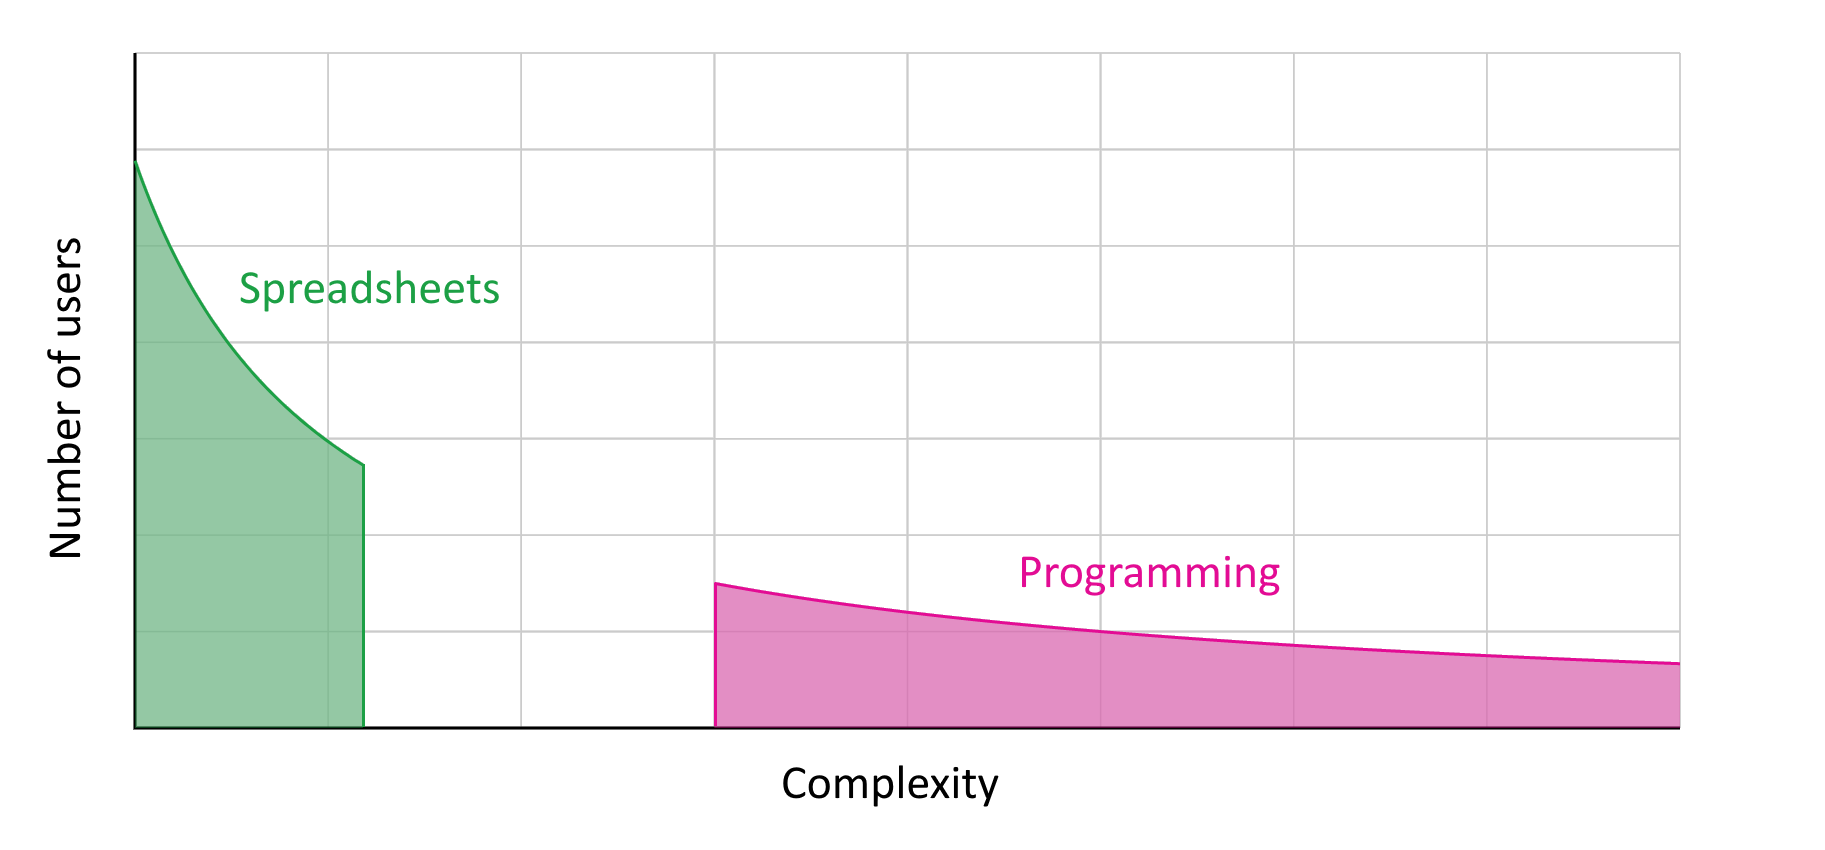
\includegraphics[scale=0.25]{img/gap.png}
\vspace{-0.5em}
\caption{Illustration showing a gap between easy to use but limited spreadsheets
and unlimited but hard to use programming tools. Adapted from \citet{edwards-2015-transcript}.}
\label{fig:gap}
\vspace{1em}
\end{figure}

The above illustration should not be taken at face value. Although there is no single accepted
solution, there are multiple projects that exist in the gap between spreadsheets and programming
tools. However, the gap provides a useful perspective for positioning the contributions presented
in this thesis. Some of the work develops novel tools that aim to combine the simplicity of
spreadsheets with the power of programming for the specific domain of data exploration, aiming to
fill the space in the middle of the gap. Some of the work I present focuses on making regular
programming with data easier, or making simple programming with data accessible to a greater
number of users, reducing the size of the gap on the side of programming.

\begin{figure}[t]
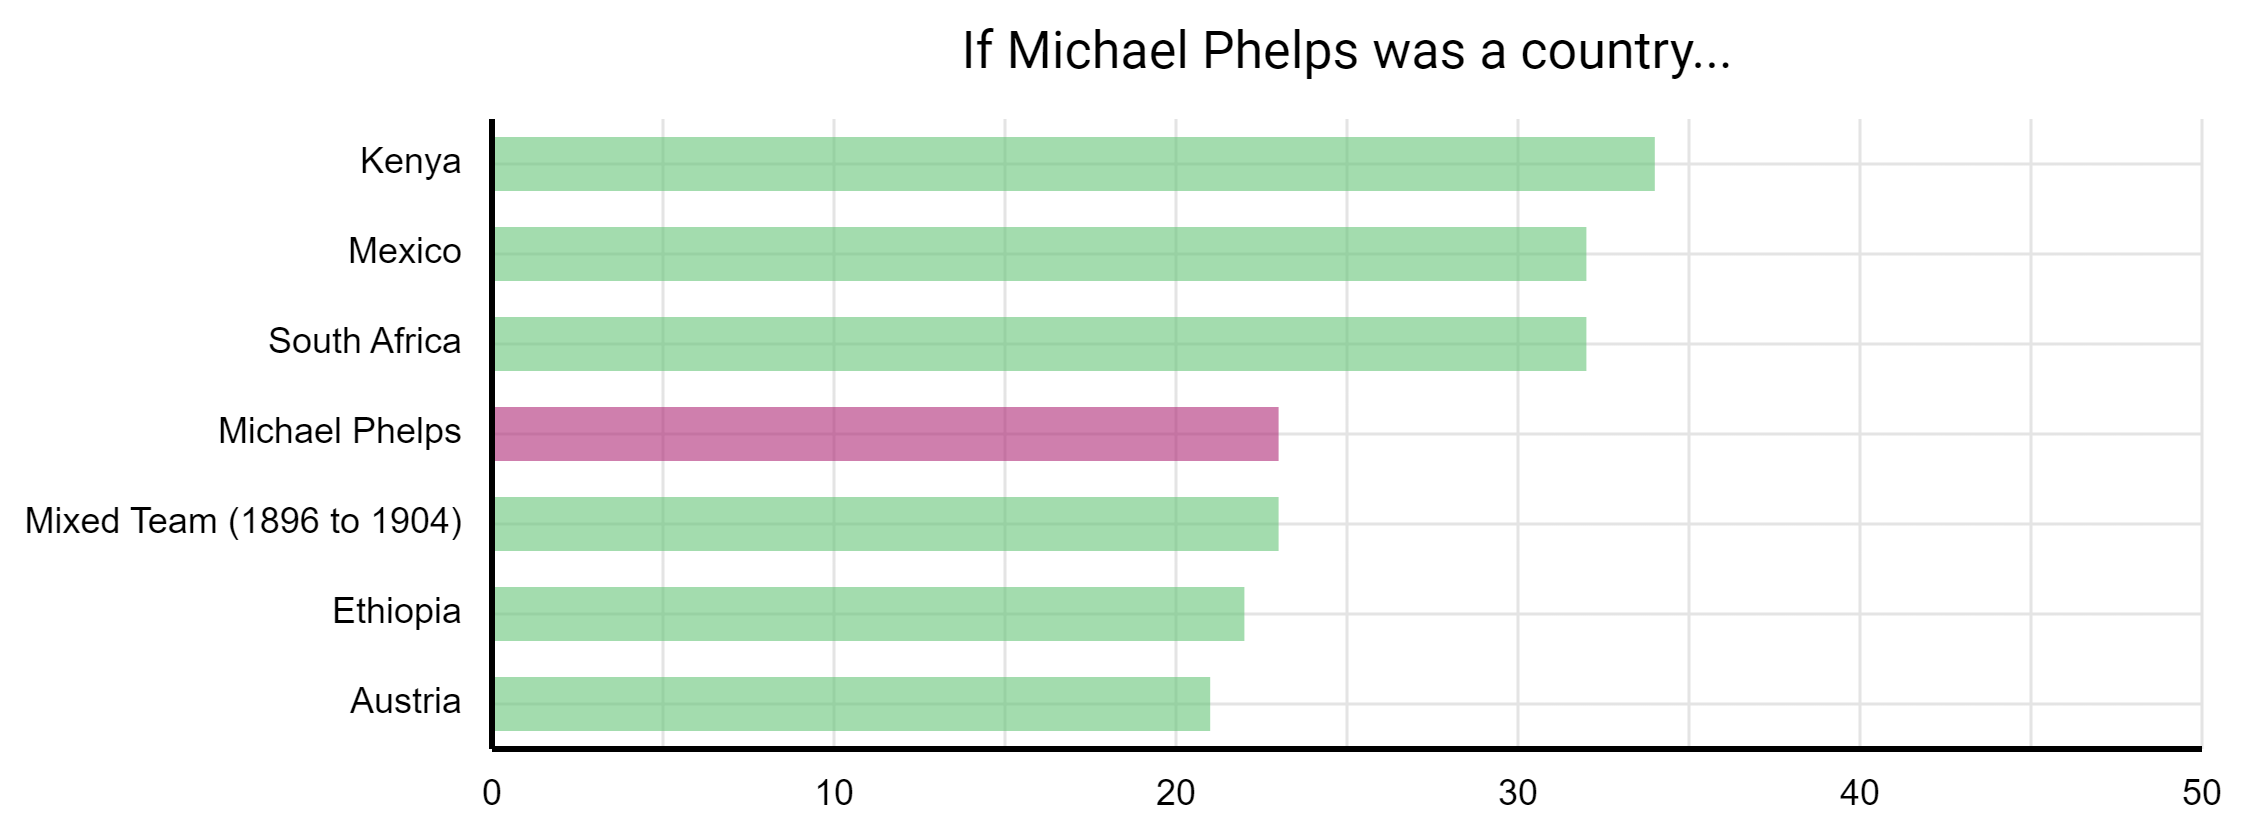
\includegraphics[scale=0.345]{img/phelps.png}
\caption{A visualization comparing the number of gold Olympic medals won by Michael Phelps
 with countries that won a close number of gold medals. Inspired by e.g., \cite{npr-2016-phelps}}
\label{fig:phelps}
\end{figure}

\section{How data journalists explore data}
To explain the motivation of this thesis, I use an example data exploration done in the context of
data journalism \citep{bounegru-2021-handbook}. Following the phenomenal success of the swimmer
Michael Phelps at the 2016 Olympic games, many journalists produced charts such as the one
in Figrue~\ref{fig:phelps}, which puts Phelps on a chart showing countries with similar number
of medals. Even such simple visualization raises multiple questions. Is the table counting
Gold medals or all medals? Would it change if we used the other metric? What would it look like
if we added more countries or removed the historical ``Mixed Team''? How many top countries
were skipped?

This simple example illustrates two challenges that I hinted at earlier. First, producing this
visualization may not be hard for a programmer, but it involves a number of tricky problems
for a non-programmer. It has to acquire and and clean the source data, aggregate medals by
country and produce and join two subsets of the data. Doing so manually in a spreadsheet
is tedious, error-prone and not reproducible, but using Python or R requires non-trivial programming
skills. Second, the non-technical reader of the newspaper article may want to answer the above
follow-up questions. Data journalists sometimes offer download of the original dataset, but the
reader would then have to redo the analysis from scratch. If the data analysis was done in Python
or R, they could get the source code, but this would likely be too complex to modify.

This thesis presents a range of tools that allow non-programmers, such as data journalists, to
clean and explore data, such as the table of Olympic medals, and produce data analyses that are
backed by source code in a simple language that can be read and understood without sophisticated
programming skills. The code can be produced interactively, by repeatedly choosing one from a
range of options offered by the tool and can then be modified to change parameters of the
visualization.

\begin{figure}[t]
\begin{thegamma}
\kvd{let} data = olympics.'group data'.'by Team'.'sum Gold'.then
    .'sort data'.'by Gold descending'.then
    .paging.skip(42).take(6)
    .'get series'.'with key Team'.'and value Gold'

\kvd{let} phelps = olympics.'filter data'.'Athlete is'.'Michael Phelps'.then
    .'group data'.'by Athlete'.'sum Gold'.then
    .'get series'.'with key Athlete'.'and value Gold'

charts.bar(data.append(phelps).sortValues(true))
    .setColors(["#94c8a4","#94c8a4","#94c8a4","#e30c94"])
\end{thegamma}
\caption{Source code of the data analysis used to produce the visualization in
Figure~\ref{fig:phelps}. The case study is based on the work presented in Chapter~\ref{ch:thegamma}.}
\label{fig:gamma}
\end{figure}

As an example, the source code of the data analysis used to produce the visualization above is shown
in Figure~\ref{fig:gamma}. The tools that enable non-programmers to create it will be discussed
later. The key aspect of the code is that it mostly consists of sequence of human-readable
commands such as \ident{'filter data'.'Athlete is'.'Michael Phelps'}. Those are iteratively
selected from options offered by the system and so the author of the data analysis can complete
most of the analysis without writing code.

The use of a simple programming language also makes it possible to understand the key
aspects of the logic. The analysis counts the number of gold medals (\ident{'sum Gold'}),
skips 42 countries before the ones shown in the visualization and does not filter out any
other data. Finally, the code can be easily executed (in a web browser), allowing the reader
to easily make small changes, such as pick a different athlete or increase the number of displayed
countries. Such engagement has the potential to aid their positive percpetion of open, transparent
data-driven insights based on facts.

\section{Requirements of simple tools for data exploration}

Although the tools and techniques presented in this thesis are more broadly applicable,
the focus of this thesis is on a narrower domain illustrated by the above motivating example.
I focus on programmatic data exploration tools that can be used to produce accessible and
transparent data analyses that will be of interest to a broader range of readers and allow
them to critically engage with the data.

In the subsequent discussion, I thus distinguish between \emph{data analysts} who produce the
analyses and \emph{readers} who consume and engage with the results. The former are
technically-skilled and data-literate, but may not have programming skills. The latter are
non-technical domain experts who may nevertheless be interested
in understanding and checking the analysis or modifying some of its attributes.
This context leads to a number of requirements for the envisioned data exploration tools:

~

\begin{itemize}
\item \emph{Gradual progression from simple to complex}. The system must allow non-program\-mers with
limited resources to easily complete simple tasks in an interface that allows them to later
learn more and tackle harder problems. In the technical dimensions of programming systems
framework \citep{jakubovic-2023-techdims}, this is described as the staged levels of complexity
approach to the learnability dimension.

\item \emph{Support transparency and openness}. The readers of the resulting data analyses must
be able to understand how the analysis was done and question what processing steps and parameters
have been used in order to critically engage with the problem.

\item \emph{Enable reproduction and learning by percolation}. A reader should be able to see and
redo the steps through which a data exploration was conducted. This lets them reproduce the results,
but also learn how to use the system. As noted by \citet{sarkar-2018-spreadsheets}, this is how
many users learn the spreadsheet formula language.

\item \emph{Encourage meaningful reader interaction}. The reader should not be just a passive
consumer of the data analyses. They should be able to study the analysis, but
also make simple modifications such as changing analysis or visualization parameters,
as is often done in interactive visualizations by journalists \citep{kennedy-2021-engagements}.
\end{itemize}

The above criteria point at the gap between spreadsheets and regular programming systems
illustrated by Figure~\ref{fig:gap} and there are multiple possible solutions and approaches to
satisfy the above criteria. This thesis explores one particular point in the design space,
which is to treat data analysis as a program with an open source code, created in a simple
programming language with rich tooling.

As I will show, treating data exploration as a programming problem makes it possible to satisfy
the above criteria. Gradual progression from simple to complex can be supported by a language
that provides very high-level abstractions (or domain-specific langauges) for solving simple
problems. Transparency, openness and reproducibility are enabled by the fact that the source code
is always available and can be immediately executed, while learning
by percolation can be supported by structuring the program as a sequence of transformations.
Finally, meaningful interaction can be offered by suitable graphical tools that simpify editing
of the underlying source code.

\section{Data exploration as a programming problem}

Data exploration is typically done using a combination of tools including spreadsheets,
programming tools, online systems and ad-hoc utilities. Spreadsheets like Excel and business
intelligence tools like Tableau \citep{wesley-2011-tableau} are often used for manual data
editing, reshaping and visualization. More complex and automated data analyses are done in
programming languages like R and Python using a range of data processing libraries such as pandas
and Tidyverse \citep{wickham-2019-tidyverse}. Such analyses are frequently done in a computational
notebook environments such as RStudio or Jupyter \citep{kluyver-2016-jupyter}, which make
it possible to interleave documentation, mathematical formulas and code with outputs such as
visualizations. Online data processing environments like Trifacta provide myriads of tools for
importing and transforming data, which are accessible through different user interfaces or
programmatic interfaces, but even those have to be complemented with ad-hoc single-purpose tools,
often invoked through a command line interface.

Finding a unified perspective for thinking about such hotchpotch of systems and tools
is a challenge. The view taken in this thesis is that, most of the systems and tools can be
considered as programming systems. This view makes it possible to apply the powerful methodology
of programming languages research to the problem of data exploration.
However, the programs that are constructed during data exploration have a number of specific
characteristics that distinguishes them from programs typically considered in programming
langauge research:

\begin{itemize}
\item \emph{Data exists alongside code}. Systems such as spreadsheets often mix
  data and code in a single environment. In conventional programming, this is done in
  image-based systems like Smalltalk, but not in the context of programming languages.

\item \emph{Concrete inputs are often known}. Moreover, data exploration is typically done on a
  known collection of concrete input datasets. This means that program analysis can take
  this data into account rather than assuming arbitrary unknown inputs.

\item \emph{Programmers introduce fewer abstractions}. Even in programmatic data exploration using
  R or Python in a Jupyter notebook, data analysts often write code as a sequence of
  direct operations on inputs or previously computed results, rather than introducing abstractions
  such as reusable generic functions.

\item \emph{Most libraries are externally defined}. Finally, data exploration is
  often done using libraries and tools that are implemented outside of the tool that the analysts
  use. For example, spreadsheet formulas use mostly built-in functions, while data analyses in
  Python often use libraries implemented in C/C++ for performance reasons.
\end{itemize}

The above generally hold for simple data explorations that are done by data journalists, public
servants and analysts that this thesis is primarily concerned with. The characteristics do not
apply to all programs that work with data, which may include complex reusable and parameterized
models, general-purpose algorithms and rich data processing pipelines. However, focusing on simple
data exploration problems for which the above criteria are true allows us to narrow the design
space and study a range of interesting problems. The narrow focus also makes us rethink a number of
accepted assumptions in programming language research, such as what are the key primitives to be
included in a formal model of a programming language (in Chapter~\ref{ch:foundations}, an
invocation of an external function becomes more important than lambda abstraction).

\section{Utilized research methodologies}
The research presented in this thesis tackles multiple research questions such as:
Does a particular language design rule out certain kinds of programming errors? What is an
efficient implementation technique for a particular langauge or a tool? Does a newly
developed tool simplify data exploration by reducing the number of manual interventions
by the user? What is a suitable interaction mechanism for completing a particular task?
And can non-programmers effectively use such interaction mechanism?
The diversity of the research questions calls for a corresponding diversity of research
methodologies.

\paragraph{Programming language theory.}
The first methodology used in this thesis is that of theoretical programming langauge research.
When using this methodology, a core aspect of a programming language is described using a small,
formally tractable mathematical model that captures the essential properties of the aspect.
The model is then used to formally study properties of the given aspect, such as whether a
programming langauge that impements it can be used to write programs that exhibit certain kind
of incorrect behaviour.

In this thesis, Part~\ref{part:providers} presents two instances of a programming language
extension mechanism called type providers. To show that code written using type providers will
never result in a particular error condition, I develop a formal model of type providers and prove
a correctness property using the model. The actual system implementation then closely follows the
formal model. Theoretical programming language research methods are also used to develop a data
visualization laguage in Chapter~\ref{ch:galois}, to formalize the optimization technique introduced
in Chapter~\ref{ch:foundations} and to define the structure of the semi-automatic data wrangling
tools developed in Chapter~\ref{ch:aia}.

\paragraph{Programming systems.}
The theoretical approach is complemented by a range of applied programming systems methods.
The work using those methodologies often focuses on designing suitable system architecture,
empirical evaluation of measurable characteristics of the system such as efficiency. It should
also be complemented with an open-source implementation and/or a reproducibe software artifact.

I use the programming systems research methodology primarily in Chapter~\ref{ch:wrattler}, which
presents the architecture and an implementation of a novel computational notebook system for data
science. Chapter~\ref{ch:foundations} develops an optimized programming assistance tool and
evaluates the efficiency empirically. Software systems and libraries presented in this thesis
are available as open-source and are listed below.

\paragraph{Human-computer interaction.}
Finally, answering questions that concern usability requires a human-centric approach offered by
the human-computer interaction (HCI) research methodology, which is increasingly used to study
programming languages and systems \citep{chasins-2021-plhci}. The HCI methods include controlled
usability studies, qualitative and quantitative user studies, as well as the development and
application of heuristic evaluation frameworks.

I use the HCI methodology in Chapter~\ref{ch:thegamma}, which introduces the ``iterative prompting''
interaction mechanism and conducts a usability study with non-programmers to evaluate whether
they can use it to complete simple data exploration tasks. Chapter~\ref{ch:compost}, which
presents a novel data visualization library, also draws on the HCI methodology, but uses a
comprehensive case study instead of a user study to evaluate the design.

\section{What makes a programming tool simple}

The very title of this thesis refers to the aim of creating programming tools for data exploration
that are \emph{simple}. However, simplicity is difficult to quantify exactly and is understood
differently by different communitites and in different contexts. I thus follow the recommendation
of \citet{muller-2020-rhetoric} to make explicit how the term should be understood in the
context of this thesis. The notion of simplicity is used as a unifying theme in this commentary,
but it takes one of several more specific and rigorously evaluable forms:

\begin{itemize}
\item In the context of user-centric work, I refer to a system as \emph{simple} if it allows
  non-programmers to complete tasks that are typically limited to programmers. This is the
  case when discussing the iterative prompting interaction principle in Chapters~\ref{ch:thegamma}
  the live programming tools in Chapter~\ref{ch:foundations}.

\item In the context of programming language or library design, I consider the design \emph{simple}
  when it allows expressing complex logic using a small set of highly composable primitives
  that are easy to understand. This applies to the language design in Chapter~\ref{ch:dotdriven}
  and visualization library design in Chapter~\ref{ch:compost}.

\item In the context of programmer assistance tools, simple indicates that the
  user does not have to perform a task that they would otherwise have to complete manually.
  This applies to AI assistants, presented in Chapter~\ref{ch:aia}, which relieve the user from
  tedious manual setting of parameters by partly automating the task.

\item Finally, I also use the term simple when talking about programming systems and libraries
  that provide a high-level interface designed specifically for a particular task. This is the
  case for the notebook system presented in Chapter~\ref{ch:wrattler}, data access library
  in Chapter~\ref{ch:fsdata} and the language for creating visualizations in Chapter~\ref{ch:galois}.
  Using such high-level abstractions means that programmers have write less code.
\end{itemize}

The overarching theme of this thesis is thus the design of programming tools for data exploration
that are simple in one or more of the meanings of the term indicated above. The focus on simplicity
aims to fill or reduce the technology gap illustrated in Figure~\ref{fig:gap} and, ultimately,
make data exploration accessible to a broader range of users.

\section{Structure of the thesis contributions}

The contributions of this thesis cover multiple different kinds of tasks that a data analyst
faces when they work with data. To position the contributions in the broader context of data
analytical work, Figure~\ref{fig:lifecycle} shows where they fit in the data science lifecycle
as defined by IBM (with slight modifications). As the diagram shows, the focus of this thesis is on work done in the
initial data exploration phase.

\begin{figure}[h]
  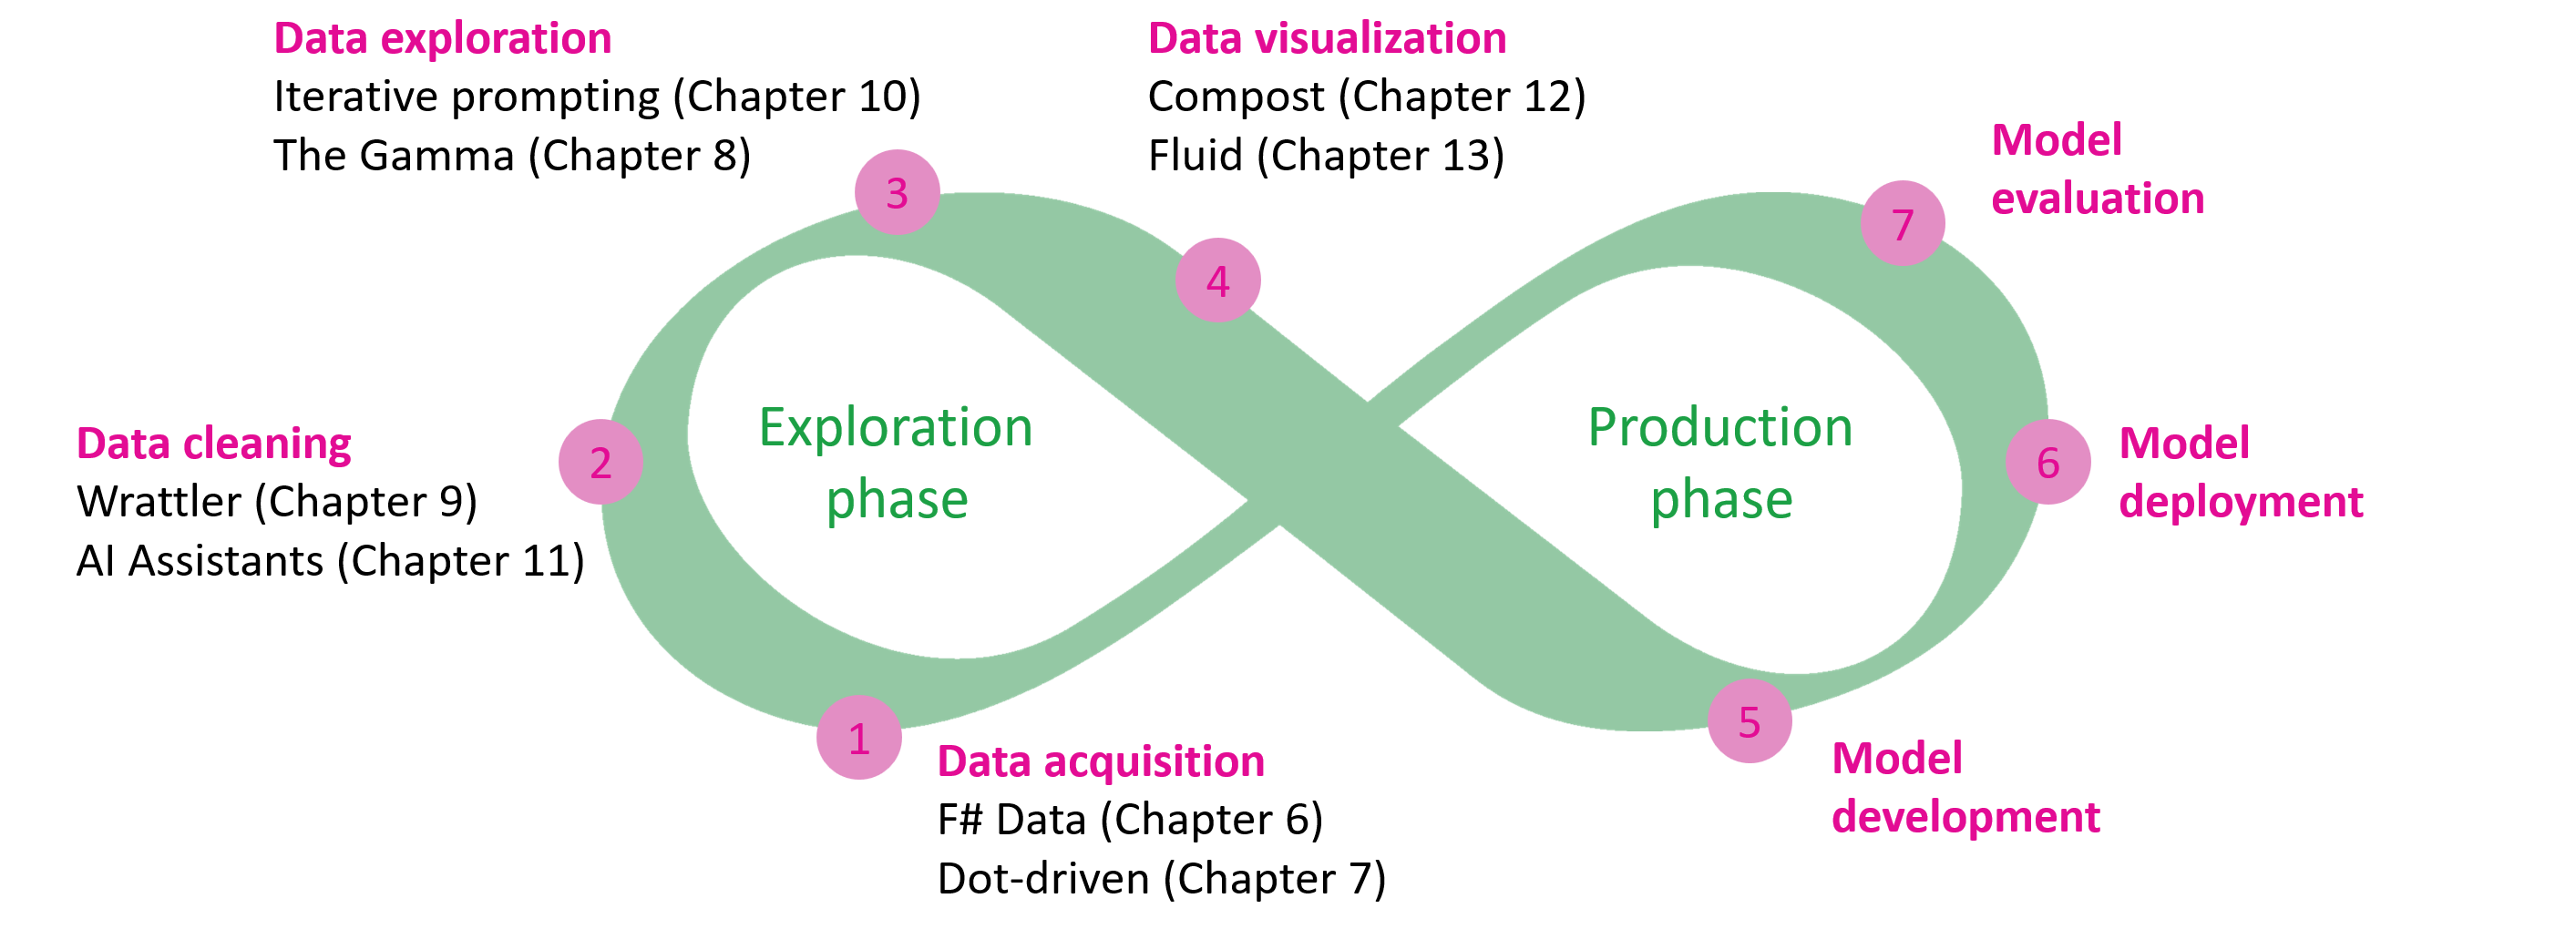
\includegraphics[scale=0.2]{img/lifecycle.png}
  \vspace{-1em}
  \caption{Illustration showing the data science lifecycle, as understood by \cite{ibm-2020-lifecycle},
  alongside with the contributions of this thesis to the individual steps of the data exploration phase.}
  \label{fig:lifecycle}
\end{figure}

The data science lifecycle starts with data acquisition (1), which involves loading
data from a range of sources. This is followed by data cleaning (2), where multiple data sources
are joined, incompete data is filled or removed and data structure is recovered.
In data exploration (3), the analyst transforms the data to discover
interesting patterns and, finally, in data visualization (4) they produce charts to present
their insights. In the production phase, the insights are then used to develop a model
that becomes a part of a production system. The process can be repeated based on the results
of the model evaluation.

The work that constitutes this thesis contributes to each of the four steps of the data
exploration phase. In Part~\ref{part:providers}, I present two papers on type providers,
which simplify data acquisition, while Part~\ref{part:visualization} consists of two
novel data visualization systems. The four publications presented in Part~\ref{part:infra}
and Part~\ref{part:iterative} all focus on working with data, including data cleaning and
exploration. They are not grouped in parts based on the lifecycle step, but based on their research
methodology. The publications in Part~\ref{part:infra} use programming systems methods to
design new infrastructure, while Part~\ref{part:iterative} introduces a novel interaction
principle and applies it to two problems, one from the domain of data exporation and one from the
domain of data cleaning. The rest of this section summarizes the contributions of the work
presented in this thesis in more detail.

\paragraph{Type providers.}
The \emph{type provider} mechanism \citep{syme-2012-providers,syme-2013-inforich} makes it possible
to integrate external data into a statically-typed programming langauge. The work presented in
Part~\ref{part:providers} presents two new type providers.

Chapter~\ref{ch:fsdata} presents a library of type providers that makes it possible to safely access
structured data in formats such as CSV, XML and JSON in the F\# programming language. The two key
research contributions of the work are, first, a novel inference mechanism that infers a type based
on a collection of sample data and, second, a formulation of a \emph{relative safety property} that
formally captures the safety guarantees offered by the system.

Chapter~\ref{ch:dotdriven} takes the idea of type providers further. It uses the mechanism not just
for data access, but for construction of SQL-like queries over tabular data. The research
contribution is a novel type provider, implemented in The Gamma system, which generates a type that
can be used to group, filter and sort tabular data. Using a novel formal model, the presented paper
shows that all queries constructed using the type provider are valid.

\paragraph{Data infrastructure.}
Programmatic data exploration is typically done in notebook systems such as Jupyter
\citep{kluyver-2016-jupyter} that make it possible to combine documentation, formulas, code and
output such as visualizations. Notebook systems are a convenient tool, but they suffer from
a number of limitations and issues. The two novel systems presented in Part~\ref{part:infra} adress
some of those.

Chapter~\ref{ch:foundations} presents a programming environment for The Gamma that makes data
exploration easier by providing instant feedback. The research contributions of the work are
twofold. First, builds a practical efficient algorithm for displaying live previews. Second, it
develops a formal model of code written to explore data called \emph{data exploration calculus}
and uses it to show the correctness of the live preview algorithnm.

Chapter~\ref{ch:wrattler} tackles more directly the problems of notebook systems. It presents
Wrattler, which is a novel notebook system that makes it possible to combine multiple
programming languages and tools in a single notebook, resolves the reproducibility issues of
standard systems and stores computation state in a transparent way, allowing for precise
data provenance tracking.

\paragraph{Iterative prompting}
Treating data analyses as programs makes them transparent and reproducible, but writing code has
an unavoidable basic complexity. Part~\ref{part:iterative} presents a novel interaction principle for
program construction called \emph{iterative prompting}. The mechanism is rooted in the work on type
providers and makes it possible to construct programs by repeatedly choosing from one of several
options.

Chapter~\ref{ch:thegamma} introduces the iterative prompting mechanism from the human-computer
interaction perspective. It shows that the mechanism can be used to construct programs that
explore data in multiple input formats including tables, graphs and data cubes. The usability of
the mechanism is evaluated through a user study, showing that non-programmers can use it to
complete a range of data exporation tasks.

Chapter~\ref{ch:aia} uses the iterative prompting mechanism as the basis of a range of
semi-automatic data cleaning tools. It augments existing AI tools for parsing data, merging data,
inferring data types and semantic information with a mechanism that lets the user guide the AI
tool. Using iterative prompting, the user can correct mistakes and configure parameters of the tool.
The augmented tools are evalauted empirically, showing that the correct result can typically be
obtained with 1 or 2 manual interventions.

\paragraph{Data visualization.}
Data visualization is the last step in the exploratory phase of the data science lifecycle
discussed above. Although standard charts are typically easy to build, creating richer
interactive visualizations is a challenging programming task. Part~\ref{part:visualization}
presents two systems that make it easier to build interactive data visualizations that encourage
critical thinking about data.

Chapter~\ref{ch:compost} presents a functional domain-specific language for creating charts that
makes it possible to compose rich interactive charts from basic building blocks (such as lines
and shapes) using small number of combinators (such overlaying and nesting of scales).
The simplicity of the approach is illustrated through a range of examples and confirmed by the
publication of the work as a so-called functional pearl \citep{gibbons-2010-pearl}.

Chapter~\ref{ch:galois} introduces a language-based program analysis technique that makes it
possible to automatically build linked data visualizations that show the relationships between parts
of charts produced from the same input data. The key research contribution is a novel bidirectional
dynamic dependency program analysis, which is formalised and shown to have a desirable formal
structure. The technique is used as the basis for a high-level programming langauge Fluid.

\section{Open-source software contributions}

The work presented in this thesis is not merely theoretical. An important contribution
of this thesis is a practical implementation of the presented programming systems, languages
and libraries. The concepts discussed in the previous section have been implemented in
several open-source software packages that are available under the permissive Apache 2.0 (F\# Data)
and MIT (all other projects) licenses.

\begin{itemize}
  \item \textbf{F\# Data} (\url{https://github.com/fsprojects/FSharp.Data}) has became a widely-used
    F\# library for data access. It implements utilities, parsers and type providers for working
    with structured data in multiple formats (XML, JSON, HTML and CSV). The initial version based
    on the work presented in Chapter~\ref{ch:fsdata} has since been extended by multiple
    contributors from the F\# community.

  \item \textbf{The Gamma} (\url{https://github.com/the-gamma}) is a simple data exploration
    environment for non-programmers such as data journalists. It implements the iterative
    prompting mechanism for data access (Chapters~\ref{ch:thegamma} and \ref{ch:dotdriven})
    and live preview mechanism (Chapter~\ref{ch:foundations}). Live demos using the environment
    in a web browser can  be found at \url{https://thegamma.net} and \url{https://turing.thegamma.net}.

  \item \textbf{Wrattler} (\url{https://github.com/wrattler}) is an experimental notebook system
    described in Chapter~\ref{ch:wrattler} that tracks dependencies between cells, makes it
    possible to combine multiple langauges in a single notebook and hosts AI assistants for
    data wrangling described in Chapter~\ref{ch:aia}. More information can be found at
    \url{http://www.wrattler.org}.

  \item \textbf{Compost.js} (\url{https://github.com/compostjs}) is a composable library for creating
    data visualizations described in Chapter~\ref{ch:compost}. Although the library is implemented
    in the F\# language, it is compiled to JavaScript and provides a convenient interface for
    Java\-Script users. A range of demos illustrating the use of the library can be found online at
    \url{https://compostjs.github.io}.

  \item \textbf{Fluid} (\url{https://github.com/explorable-viz/fluid}) is a programming langauge
    for building linked data visualizations described in Chapter~\ref{ch:galois}. The project has
    since been developed into a general-purpose langauge for transparent, self-explanatory research
    outputs by the Institute of Computing for Climate Science, University of Cambridge.
    A live example can be found at \url{https://f.luid.org}.
\end{itemize}

\chapter{Type providers}

Accessing data has traditionally been easier in dynamically typed scripting languages,
because the language does not need to consider the structure of the input data when
checking if the program accesses it correctly. The type provider mechanism, originally
implemented in F\# \citep{syme-2012-providers,syme-2013-inforich} makes it possible to achieve
similar simplicity with static type checking by providing an extension -- a type provider -- that
infers types based on external inputs. The provided types are then used to check

\chapter{Data infrastructure}
\chapter{Iterative prompting}

\cite{rattenbury-2017-wrangling}
50-80
with messy data. Surveys \cite{kaggle-2017-state} indicate
that up to 80\% of data engineering is spent on \emph{data wrangling}, a tedious process of

\chapter{Data visualization}

what?
what?


\part{Publications: Type providers}
\label{part:providers}

\chapter{Types from data: Making structured data first-class citizens in F\#}
\label{ch:fsdata}

\chapter{Data exploration through dot-driven development}
\label{ch:dotdriven}

\part{Publications: Data infrastructure}
\label{part:infra}

\chapter{Foundations of a live data exploration environment}
\label{ch:foundations}

\chapter{Wrattler: Reproducible, live and polyglot notebooks}
\label{ch:wrattler}

\part{Publications: Iterative prompting}
\label{part:iterative}

\chapter{The Gamma: Programmatic data exploration for non-programmers}
\label{ch:thegamma}

\chapter{AI Assistants: A framework for semi-automated data wrangling}
\label{ch:aia}

\part{Publications: Data visualization}
\label{part:visualization}

\chapter{Composable data visualizations}
\label{ch:compost}

\chapter{Linked visualisations via Galois dependencies}
\label{ch:galois}

\part{Conclusion}

\chapter{Contributions}

thanks
who did what
(especially galois)

\chapter{Conclusion}

if the society is to benefit...

AI and LLMs

in other words, technology has democratized opinions, but can it also democratize facts

























% Bibliography
\bibliographystyle{ACM-Reference-Format}
%\bibliographystyle{abbrv}
\bibliography{thesis}

\end{document}
